\section{Visualisation}
%what are the features we want to emphasis?
%make a bullet list of something like that
Our goal is to design an interactive visualisation system on top of the structured prediction framework.
Figure~\ref{fig:overview} shows the overview of a live demo system, which consists of four major components: a map to display suggested routes, an input box for user query on the left side, a stacked score of routes on the upper right side, and a radar chart to compare multiple POIs on the lower right side. 
The role and the construction of three major components, except the main map, are as follow:

%\begin{itemize}
\textbf{Query input}: A query consists of a starting POI and a trip length. 
Users can choose the starting POI by clicking icons on the map and can adjust the slide to set the trip length. 
In addition, we support three different travelling modes: bicycling, walking, and driving.
Based on the different mode, we optimise suggested routes between POIs in a sequence.

\textbf{Route score visualisation}: Ranks of candidate routes are determined by the total scores from the SSVM. 
The score of each route can be decomposed into each POI and edge scores along the route. 
We adopt the LineUp framework~\cite{gratzl2013lineup} designed to support the visualisation of multi-attribute ranking via stacked representation. 
Figure~\ref{fig:stack} shows the stacked representation of the top ten scored routes, where the proportion of each bar indicates the importance of each POI in the route.

\textbf{POI feature visualisation}: We further provide a tool to analyse the variation between POIs in a single route. 
For example, in Figure~\ref{fig:radar}, we compare two POIs, the Queen Victoria Market and Melbourne Aquarium, in terms of POI features and their importance in the suggested route. 
%\end{itemize}

\begin{figure}[t!]
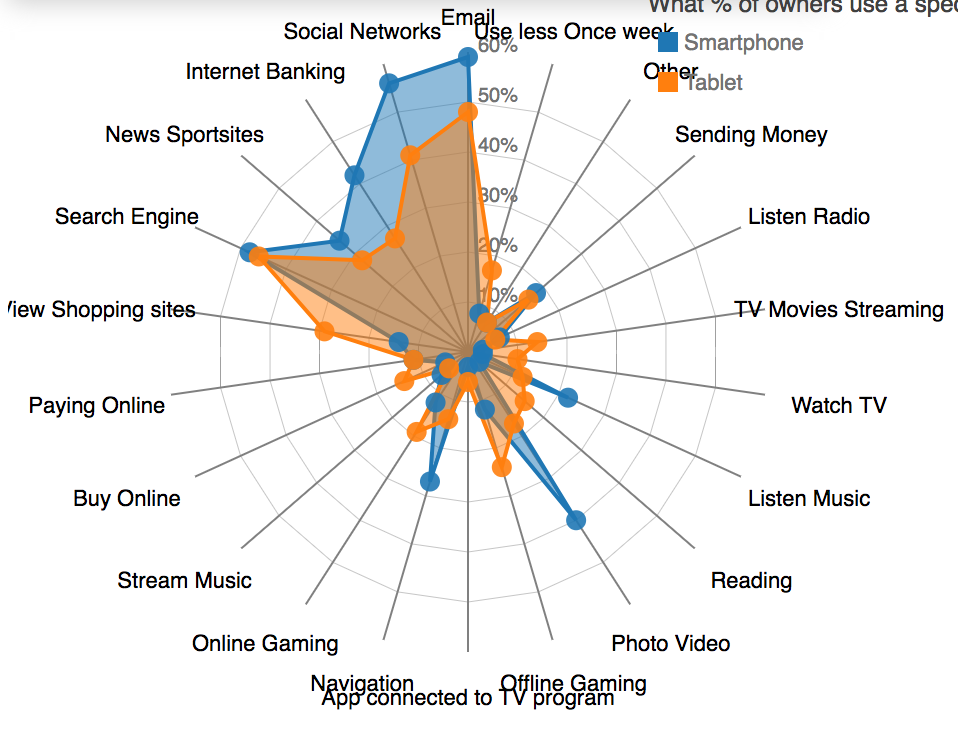
\includegraphics[width=0.8\linewidth]{figure/sample_radar.png}
\caption{Comparison between the Queen Victoria Market and Melbourne Aquarium. The Queen Victoria Market has a high score on \textit{shopping} and \textit{city precincts} features whereas the Melbourne aquarium has a high score on \textit{Entertainment} feature.}
\label{fig:radar}
\end{figure}